\chapter{Evaluation}
\label{chap:evaluation}

This chapter evaluates the methodology proposed in Chapter~\ref{chap:methodology} by applying the implementation described in Chapter~\ref{chap:implementation}. The objective is to empirically assess whether an Active Inference (AIF) agent can dynamically control computational elasticity to uphold Service Level Objectives (SLOs) while maximizing Quality of Experience (QoE) in edge computing environments. To provide a grounded comparison, we contrast the AIF agent with a simple heuristic agent under three controlled scenarios: a stable baseline, variable computational demand, and fluctuating computational budget. Each scenario simulates different real-world challenges encountered in distributed edge deployments, such as load bursts, resource contention, and partial node failure.

\section{Baseline: Threshold Based Control Agent}
\label{sec:evaluation-heuristic}

To evaluate the effectiveness of the Active Inference approach, we implement a baseline agent based on a fixed threshold (heuristic) policy. Threshold-based autoscaling is the most widely adopted control strategy in both academic and industrial settings~\cite{arabnejad_comparison_2017}, including platforms such as Amazon EC2~\cite{noauthor_amazon_nodate}, Microsoft Azure~\cite{noauthor_cloud_nodate}, OpenStack~\cite{noauthor_open_nodate}, and Kubernetes~\cite{noauthor_production-grade_nodate}. Their simplicity, transparency, and widespread deployment make them a well-established baseline for evaluating more sophisticated, model-based control schemes.

The agent operates reactively based on SLO values observed during runtime. Whenever an SLO violation is detected, the heuristic agent adjusts stream parameters with the highest capacity. If the parameters have the same capacity, the decreasing action is taken according to a predefined order of importance: first reducing the inference quality, then the fps, and finally the resolution. When all SLos are overfullfilled, i.e., \(\text{SLO-Value} < 0.85\) and the current configuration is not maximal, it incrementally scales the quality parameters back up in the same order.
When the SLOs are fulfilled but too close to the critical threshold, i.e., \(0.85 \leq \text{SLO-Value} \leq 1\), no action is taken.

The heuristic agent does not use a generative model or perform any probabilistic inference. It cannot anticipate future states or reason under uncertainty. This makes it inherently limited to short-term, reactive control decisions. Despite its simplicity, this agent serves as a relevant baseline for highlighting the benefits of model-based adaptation under the Active Inference framework. The comparison focuses on control stability, responsiveness, and long-term QoE.

\section{Experimental Setup}
\label{sec:evaluation-setup}

\subsection{Environment}
\label{sec:evaluation-environment}

All experiments are conducted in a simulated edge computing environment using the prototype implementation described in Chapter~\ref{chap:implementation}. The system processes a live video stream of highway traffic using YOLOv11 inference for vehicle detection. The stream is segmented into frames by the producer and distributed to workers for parallel processing. The collector assembles the results into a final output stream.

Each worker simulates a bounded compute capacity by artificially delaying inference based on a configurable slowdown factor. The producer uses SLOs to track system state and controls three stream parameters: FPS, resolution, and inference quality. The experiments are run with both the AIF agent and the heuristic baseline to allow direct comparison.

Metrics are sampled continuously and include SLO values and Stream quality parameters (FPS, resolution, inference quality). Each experiment lasts 450 seconds.

\subsubsection{Hardware and Software}
All simulations are executed in a controlled single-machine environment to ensure reproducibility and eliminate variance introduced by distributed hardware. The system configuration is as follows:

\begin{table}[H]
\centering
\caption{Hardware and Software Configuration}
\label{tab:hardware-software}
\begin{tabular}{@{}ll@{}}
\toprule
\textbf{Component} & \textbf{Specification} \\
\midrule
Operating System & Windows 11, Version 23H2 (Build 22631.5335) \\
Python Runtime & Python 3.12.2 \\
CPU & AMD Ryzen 7 7800X3D (8 cores, 16 threads) \\
GPU & Nvidia GeForce GTX 1660Ti (MSI GTX Ti Ventus XS OC) \\
GPU Driver Version & 576.88 \\
Installed CUDA Version & 12.9 \\
CUDA Compiler Version & 12.6 (cuda\_12.6.r12.6/compiler.34841621\_0) \\
Memory & 32\,GB DDR5 RAM @ 4800\,MHz (dual channel) \\
Storage & WD Black SN770 2\,TB NVMe SSD \\
\bottomrule
\end{tabular}
\end{table}


This configuration provides sufficient headroom for parallel task execution and GPU-accelerated inference, while reflecting performance characteristics common in high-end edge servers and developer workstations.

\subsection{Scenario A: Base Case}
\label{sec:evaluation-base}

This scenario evaluates agents' behavior in a stable and controlled environment. It serves as the baseline to assess the steady-state behavior of both agents. The goal is to analyze convergence behavior, control stability, and SLO compliance in the absence of external perturbations.

The experiment is conducted using three worker nodes, each assigned a fixed computational capacity of 60\%, 50\%, and 40\%, respectively

These normalized capacity values simulate processing slowdowns by artificially extending inference time. The capacities are deliberately unequal to reflect the heterogeneity typical of real-world edge environments, where nodes differ in hardware capabilities, energy budgets, or concurrent workloads.

A single video stream is processed at a constant source frame rate. At the beginning of the experiment, the system is initialized with the highest possible configuration: 30 FPS, 1080p resolution, and the YOLOv11m model. This starting point is intentionally unsustainable under the given compute constraints and is expected to trigger elastic adaptation by the controller. The goal is to evaluate whether the AIF agent reaches optimal QoE faster, switches less frequently, and maintains fewer SLO violations compared to the heuristic agent.

\subsection{Scenario B: Variable Computational Demand}
\label{sec:evaluation-variable-demand}

This scenario simulates a dynamic workload by varying the number of concurrent video streams during runtime. Three workers are assigned fixed computational capacities of 80\%, 75\%, and 70\%, respectively. The producer initiates multiple streams during a certain stream multiplier schedule, at key points during the runtime:

\begin{figure}[h!]
\centering
\scalebox{1.0}{
\begin{tikzpicture}[>=latex, thick, font=\small]
    \begin{axis}[
        width=0.8\textwidth,
        height=6cm,
        xlabel={Runtime (\%)},
        ylabel={Number of Concurrent Streams},
        xtick={0,20,40,60,80,100},
        ytick={1,2,3},
        ymin=0.5, ymax=3.5,
        xmin=0, xmax=100,
        grid=both,
        axis lines=left,
        tick label style={font=\small},
        label style={font=\small},
    ]

    \addplot[
        mark=none,
        color=blue,
        thick,
        const left
    ] coordinates {
        (0,1)
        (20,1)
        (20,2)
        (40,2)
        (40,3)
        (60,3)
        (60,2)
        (80,2)
        (80,1)
        (100,1)
    };

    \end{axis}
\end{tikzpicture}
}
\caption{Step-wise stream multiplier schedule for Scenario B: Variable Computational Demand.}
\label{fig:stream-schedule}
\end{figure}


Each stream is identified by a unique \texttt{stream\_key} and processed independently through the same distributed pipeline. The worker nodes receive tasks from all streams interleaved and must process them within their capacity constraints.

The purpose of this scenario is to evaluate how quickly and effectively the AIF and heuristic agents adapt to abrupt changes in computational demand. It also assesses the system’s ability to reconfigure quality parameters across multiple streams in parallel without violating SLOs.

\subsection{Scenario C: Variable Computation Budget}
\label{sec:evaluation-variable-budget}

This scenario evaluates controller robustness under fluctuating compute resources. The system starts with two active workers, each with 50\% compute capacity. At 33\% of the runtime, one worker is deactivated, effectively halving the available compute budget. At 66\%, the worker is reactivated, returning to the original resource budget.

This emulates a temporary node failure. The producer continues to generate tasks during the outage period, and the controller must react by reducing quality parameters to avoid SLO violations.

This scenario evaluates the ability of the AIF agent to learn the new transition dynamics during the temporary failure and to revert to a higher-quality configuration once resources are restored. The heuristic controller, by contrast, reacts only to observable SLO violations and does not model temporal dependencies.

\section{Results}

This section presents and interprets the results of the evaluation comparing an Active Inference (AIF) based agent with a baseline heuristic controller across three simulation scenarios. The analysis focuses on five core metrics that quantify SLO compliance, system stability, and output stream quality. Results are presented comparatively and are followed by a summary table aggregating the main findings.

The complete results, including all measured metrics and plots, are provided in the results section of the appendix~\ref{appendix:chap:simulation-results}.

\subsection{Evaluation Metrics and Their Significance}

The evaluation uses the following five metrics to interpret the viability and performance of the approach:

\begin{itemize}
  \item \textbf{Time All SLOs Met Simultaneously}: Fraction of time where no SLO was violated. Higher values indicate better global SLO satisfaction.
  \item \textbf{Average SLO Fulfillment Rate}: Average percentage of individual SLOs fulfilled at each timestep. This is less strict and captures partial fulfillment.
  \item \textbf{Average Stream Quality Score}: Average quality of the stream (resolution, FPS, YOLO model quality). Higher scores imply better Quality of Experience (QoE).
  \item \textbf{Maximum SLO Violation Streak}: Longest uninterrupted sequence of time steps during which at least one SLO was violated. Lower values reflect faster adaptation.
  \item \textbf{Timesteps to Reach Stable Configuration (Coefficient)}: Normalized convergence time to a stable configuration. Lower values reflect faster convergence.
\end{itemize}

An overview of the metrics is provided in table~\ref{tab:results_summary}.

\begin{table}[h!]
\centering
\caption{Summary of Core Evaluation Metrics}
\label{tab:results_summary}
\begin{tabular}{@{}lllll@{}}
\toprule
\textbf{Scenario} & \textbf{Metric} & \textbf{AIF} & \textbf{Heuristic} & \textbf{$\Delta$} \\
\midrule
\multirow{5}{*}{Base} & Time All SLOs Met & 0.983 & 0.986 & -0.28\% \\
& Avg. SLO Fulfillment & 0.994 & 0.995 & -0.08\% \\
& Stream Quality Score & 0.800 & 0.739 & +8.30\% \\
& Max SLO Violation Streak & 15 & 10 & +50.00\% \\
& Timesteps to reach stable config coeff. & 1.0 & 0.8 & +33.33\% \\
\midrule
\multirow{5}{*}{Budget} & Time All SLOs Met & 0.967 & 0.954 & +1.37\% \\
& Avg. SLO Fulfillment & 0.987 & 0.985 & +0.26\% \\
& Stream Quality Score & 0.672 & 0.754 & -10.90\% \\
& Max SLO Violation Streak & 23 & 16 & +43.75\% \\
& Timesteps to reach stable config coeff. & 1.0 & 0.9 & +11.11\% \\
\midrule
\multirow{5}{*}{Demand} & Time All SLOs Met & 0.906 & 0.902 & +0.49\% \\
& Avg. SLO Fulfillment & 0.960 & 0.971 & -1.07\% \\
& Stream Quality Score & 0.657 & 0.813 & -19.23\% \\
& Max SLO Violation Streak & 77 & 28 & +175.00\% \\
& Timesteps to reach stable config coeff. & 1.0 & 1.0 & +3.85\% \\
\bottomrule
\end{tabular}
\end{table}


\subsection{Scenario A: Base Case}

In the base scenario, both agents performed similarly in terms of SLO compliance. The AIF agent achieved a simultaneous SLO fulfillment of \(98.3\%\), marginally below the heuristic's \(98.6\%\), a relative drop of \(-0.28\%\). Likewise, the average SLO fulfillment slightly decreased from \(99.5\%\) (heuristic) to \(99.4\%\) (AIF), a negligible difference of \(-0.08\%\).

However, the AIF agent produced a significantly higher \textbf{stream quality score} (\(0.800\) vs. \(0.739\)), reflecting a relative increase of \(+8.30\%\). This demonstrates the agent’s preference for consistent high-quality configurations once an equilibrium is reached.

The \textbf{maximum SLO violation streak} increased from \(10\) to \(15\) timesteps (+50.00\%), and the convergence time increased by 33.33\%, indicating that the AIF agent performs more deliberate adaptation. This behavior aligns with the principle of epistemic exploration followed by convergence to a stable state.

\subsection{Scenario B: Variable Computational Demand}

In this scenario, the system experiences fluctuating resource availability. The AIF agent outperformed the heuristic in SLO compliance: \(96.7\%\) of time with all SLOs fulfilled versus \(95.4\%\) for the heuristic (+1.37\%), and an average SLO fulfillment of \(98.7\%\) versus \(98.5\%\) (+0.26\%).

However, this came at the cost of stream quality. The AIF agent yielded a \textbf{stream quality score} of \(0.672\), compared to \(0.754\) for the heuristic, a reduction of \(-10.90\%\). Although the agent's preference for maximizing the stream quality score and fulfilling SLOs remains the same, it still indicates a bias toward maintaining SLO satisfaction under resource constraints. 

This is reflected in figure~\ref{fig:evaluation-demand-slo-values-comparison}, illustrating the evolution of SLO values, while Figure~\ref{fig:evaluation-demand-metrics-comparison} shows the corresponding system metrics. The Active Inference agent responds promptly to increased computational demand when a second stream is introduced and effectively prevents an SLO violation upon the addition of a third stream. However, it exhibits a conservative adjustment behavior when the number of active streams is reduced, hesitating to restore stream quality parameters.

\begin{figure}[h]
    \centering
    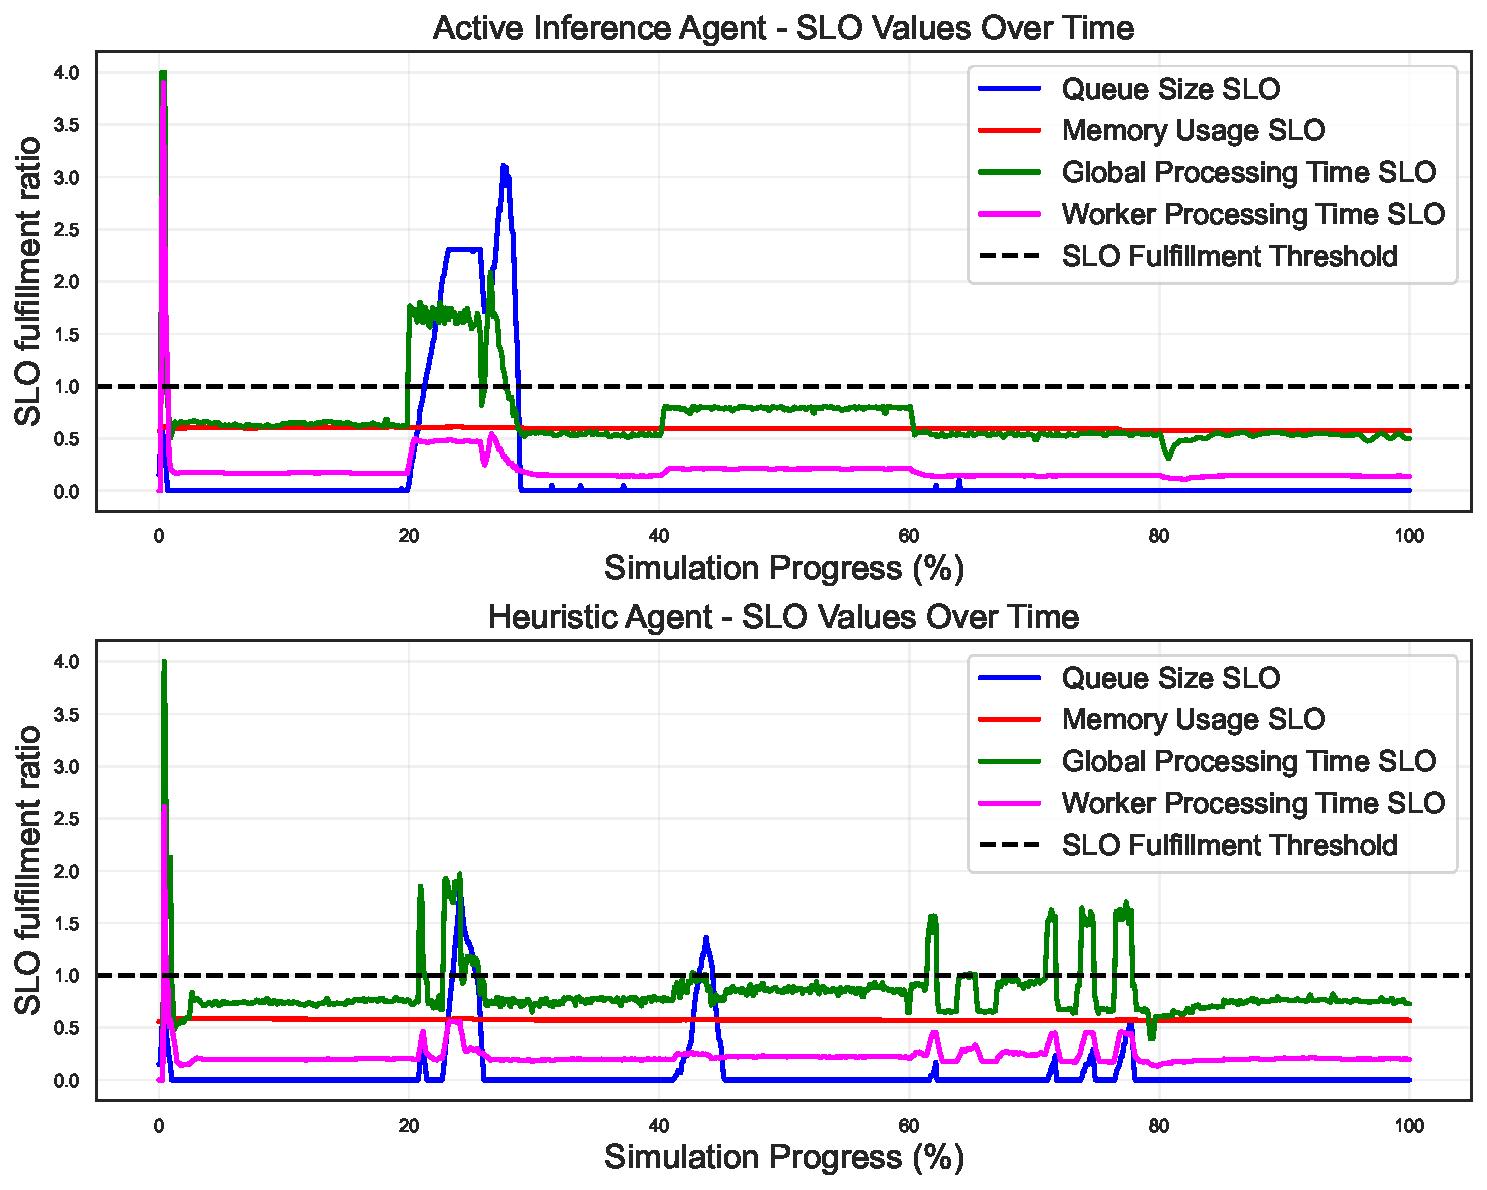
\includegraphics[width=\textwidth]{img/results/variable_computational_demand/none_combined_slo_values.pdf}
    \caption{Scenario B: Variable Computational Demand -- SLO values}
    \label{fig:evaluation-demand-slo-values-comparison}
\end{figure}

\begin{figure}[h]
    \centering
    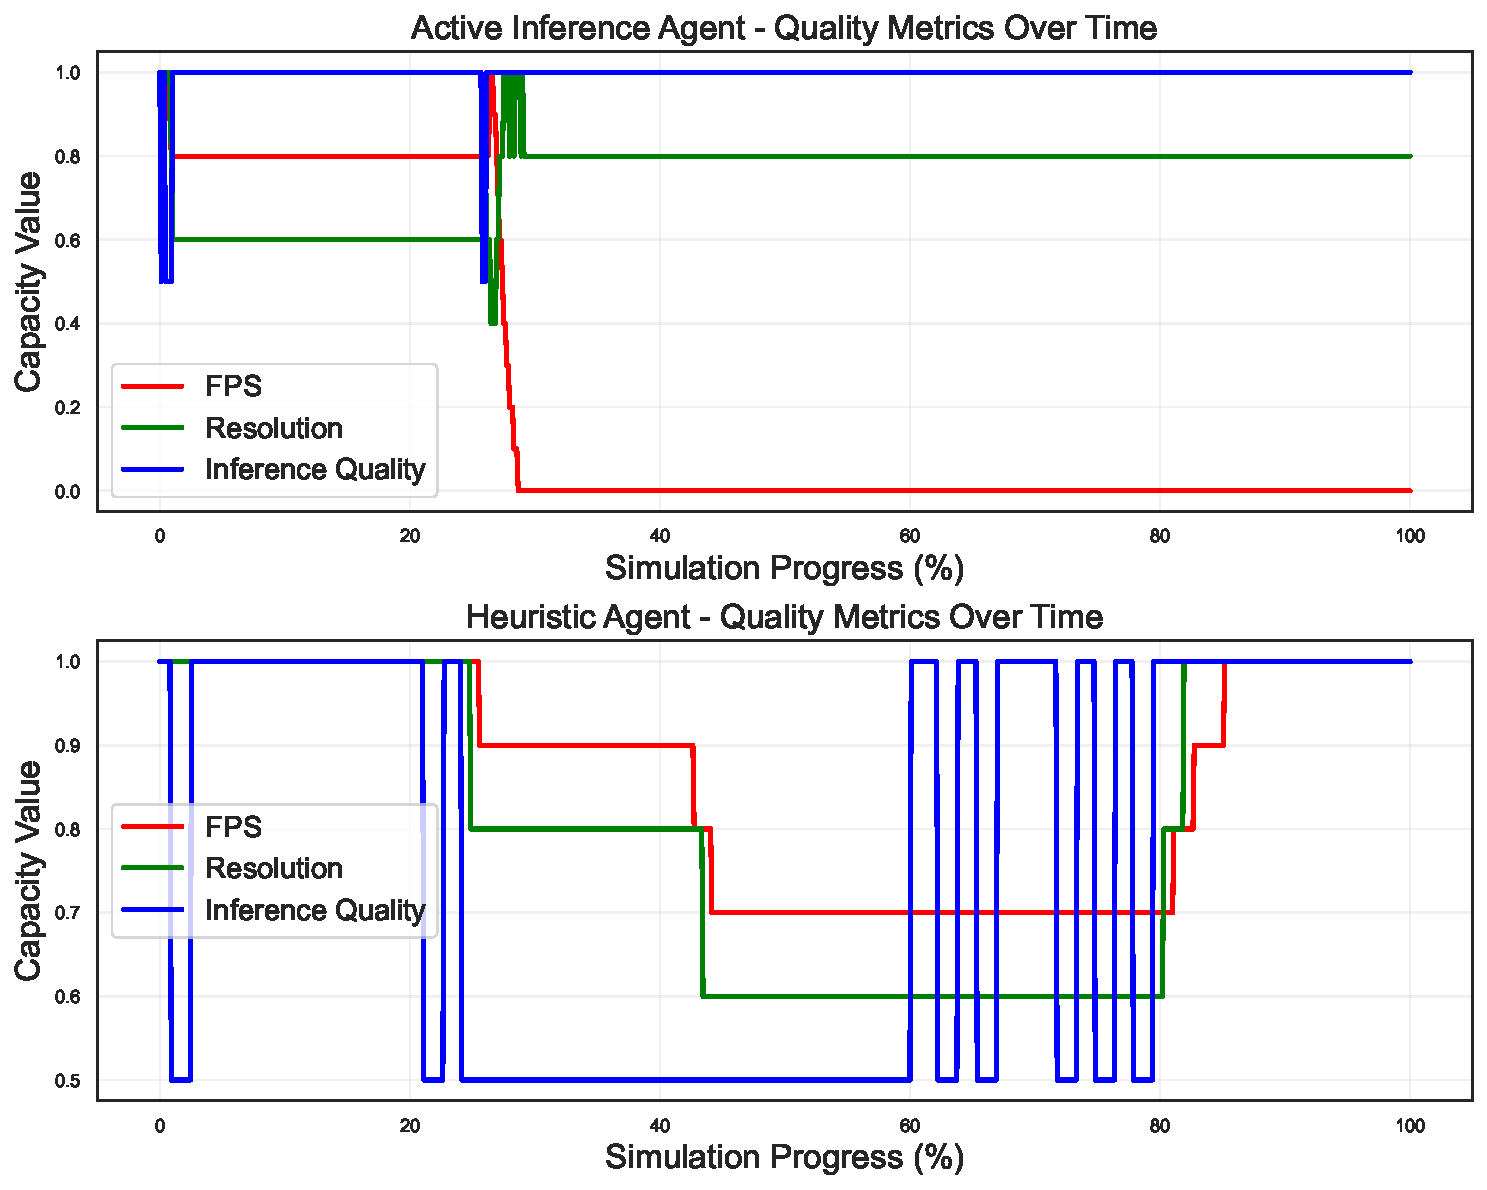
\includegraphics[width=\textwidth]{img/results/variable_computational_demand/none_combined_quality_metrics.pdf}
    \caption{Scenario B: Variable Computational Demand -- Quality Score}
    \label{fig:evaluation-demand-metrics-comparison}
\end{figure}


The maximum violation streak increased from \(16\) to \(23\) timesteps (+43.75\%), and convergence took slightly longer (+11.11\%). These effects highlight a tradeoff: higher global SLO assurance at the expense of transient responsiveness and quality.

\subsection{Scenario C: Variable Computational Budget}
This scenario involved a tripling of concurrent streams, inducing substantial load variation. Here, both agents were close in performance: AIF scored slightly better in full SLO compliance (\(90.6\%\) vs. \(90.2\%\), \(+0.49\%\)), but lower in average SLO fulfillment (\(96.0\%\) vs. \(97.1\%\), \(-1.07\%\)).

The AIF agent had a much lower \textbf{stream quality score} of \(0.657\) compared to \(0.813\) for the heuristic (\(-19.23\%\)), reflecting conservative quality selection under pressure. It also suffered a significantly higher \textbf{maximum violation streak} of \(77\) timesteps vs. \(28\) (+175.00\%), indicating an aversion to drastic changes in configuration, if a state of equilibrium was reached previously.

\subsection{Temporal Adaptation Analysis}
Across all scenarios, the AIF agent demonstrates a distinct temporal adaptation pattern: it performs early exploration (action-perception cycles), then rapidly settles into a stable configuration. Oscillation is minimal unless a significant environmental change occurs. This behavior is evidence of the AIF agent's epistemic inference structure: it avoids unnecessary changes once it has learned a suitable generative model.

The heuristic, by contrast, continuously reacts to short-term load changes. This causes frequent parameter fluctuations, sometimes leading to overuse of resources and SLO violations, despite a temporarily higher stream quality score.


\subsection{Discussion of Agent Strategies}
The AIF agent excels in scenarios with moderate or slowly varying dynamics. Its epistemic structure enables proactive stabilization, leading to consistent performance and efficient adaptation. However, the same structure hinders adaptation in high-volatility settings, where reliance on prior beliefs prevents timely reaction to rapid environmental changes.

The heuristic agent lacks a generative model and instead exploits current conditions. This results in better responsiveness but lower consistency and robustness to SLO violations. Notably, the AIF agent’s conservative behavior often sacrifices stream quality to ensure constraint adherence, aligning with its goal of minimizing long-term free energy.

These findings highlight the AIF agent's strength in sustainable system regulation, particularly in environments with moderate or gradually changing conditions. However, its limitations become apparent in highly dynamic scenarios, where reliance on prior beliefs delays necessary adaptations. Addressing this may require enhancements such as online learning or dynamic model updates to maintain responsiveness under rapidly shifting demands.